\documentclass[spanish]{udpreport}
\usepackage[utf8]{inputenc}
\usepackage[spanish]{babel}

% Podemos establecer el logo de alguna entidad o dejar el de la UDP (defecto)
%\setlogo{EITFI}

\title{Informe de redes de datos 2\\
"Levantamiento de topología física y lógica"\\}
\author{Alumno: Camilo Araya
\\Profesor: Nicolás Hidalgo\\Ayudante: Martín Griño}
\date{3 de septiembre de 2017}

% Además podemos establecer la facultad y escuela
% los valores por defecto son los siguientes:
%\udpschool{Escuela de Informática y Telecomunicaciones}
%\udpfaculty{Facultad de Ingeniería}
%\udpuniversity{Universidad Diego Portales}

\begin{document}
\maketitle

\chapter*{Resumen} 
\addcontentsline{toc}{section}{Resumen} 
\markboth{RESUMEN}{RESUMEN} 

El presente informe tiene por objetivo construir y analizar múltiples topologías de red existentes en la actualidad, por consiguiente es de vital importancia el dominio de algunos de los software orientados a un análisis integrado de red, unos de los software recomendados para el curso es el packet tracer, con el cual no solo modelaremos si no que también simularemos el funcionamiento de enviar paquetes de datos entre dispositivos en un entorno de red.
\\[0.5cm]
A continuación se presentaran los tópicos a abordar:
\\[0.5cm]
1) Construcción y funcionamiento de topologías de red entregadas por el ayudante.
\\[0.2cm]
2) Análisis de la topología de red correspondiente a la sala de informática.
\\[0.2cm]
3) análisis de la topología de red correspondiente a la sala de telemática.
\\[0.2cm]
4) solución de las preguntas de cuestionario.
\\[0.2cm]
\tableofcontents
\chapter{Introducción}
La topología de red corresponde a un orden estructurado y lógico de distintos dispositivos(computadores, impresoras, router,etc.) que logran enlazar e interconectarse en un medio de comunicación en común. Por lo general estos dispositivos a los cuales denominaremos nodos se unen mediante el uso de medios físicos como cables de red o también el uso de medios inalámbricos conocidas como antenas emisoras.
\section{Arquitectura de red}
su base radica en dos conceptos claves: topología física y lógica.
\subsection{Topología física}
Corresponde a la disposición real de los cables correspondiente a los medios como la "MAC" de un dispositivo.
\subsection{Topología lógica}
Esta define el ordenamiento de los anfitriones a la red, su utilidad radica en las redes inalámbricas y funcionan bajo el mismo criterio de las topologías físicas, trabaja a niveles de "IP". Las topologías lógicas mas comunes conocidas son las broadcast y las de transmisión de tokens.
\section{Tipos de topologías}
Esquema que representa la disposición en la cual se montan  los dispositivos o nodos creando conexiones de comunicación entre todos los participantes de la red.
\\[0.2cm]
\begin{figure}[h]
    \centering
    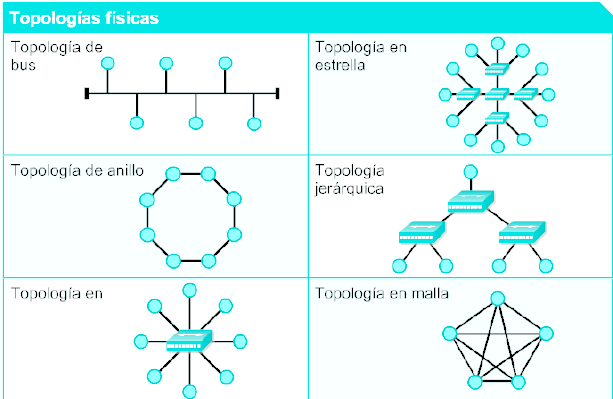
\includegraphics[scale=0.4]{images/01.png}
    \caption{Topologías Mas usadas en redes.}
    \label{fig:my_label}
\end{figure}
\newpage
\chapter{Marco teórico}
\section{Análisis topologías}
Topología troncal:Se caracteriza por un cable de red troncal el cual contiene en sus extremos dispositivos denominados terminadores que evitan la saturación de la red.
\\[0.2cm]
Topología anillo: Cada nodo tiene una única conexión de entrada/salida y están todos los nodos conectados, si falla uno de los nodos u una de las rutas se corta la comunicación en su totalidad.
\\[0.2cm]
Topología estrella: Todos los nodos están conectados a un concentrador, este es el diseño mas usado para las redes LAN, si falla el concentrador falla todo el sistema.
\\[0.2cm]
Topología estrella extendida: es similar a la topología estrella solo con una salvedad, el concentrador se distribuye en sub-concentradores, esto amplifica la red.
\\[0.2cm]
Topología de árbol:Es una variación de topología de bus, pero ramificada como una topología de estrella.
\\[0.2cm]
Topología de malla: Tiene un alto costo pero es la de mayor eficiencia en cuanto a la comunicación de red nos referimos dado que si falla un nodo no se interrumpe la conexión.
\\
\section{Hardware de red}
Son útiles para cuando se quiera construir una red, ampliar la red o mejorar el rendimiento de la red.
\\[0.2cm]
Repetidor: Útil parar expandir la red, limpiar y amplificar las señales permitiendo el aumento de nodos a la red.
\\[0.2cm]
Hub: Es un repetidor con multipuertas por lo general se utilizan como concentradores de red.
\\[0.2cm]
Bridgets: actúa en niveles de capas de enlace, elimina los tráficos innecesarios y evita los dominios de colisiones.Poseen algoritmos que lo hacen mas inteligente que un dispositivo repetidor,esto debido a que transmiten los datos a través de segmentos.
\\[0.2cm]
Switch: Es un bridgets con multipuertas, transmite tramas de datos a altas velocidades conectando en forma eficiente los segmentos de red, poseen memoria interna la cual esta compuesta por múltiples algoritmos el cual permite que este dispositivo sea uno de los mas usados en la actualidad.
\\[0.2cm]
Router:Este conecta a nivel de redes, actúa bajo la topología lógica recibiendo los frames, ubicando la dirección de envió para posteriormente enviar la información por la ruta mas óptima. Estos dispositivos realizan el enlace entre la red y el ISP ethernet(operadores locales).
\section{Colisiones de datos}
Por lo general existen problemas en extravió de datos o paquete de datos dañados al momento de usar medios de comunicación a nivel de red, a estos problemas se le denominan colisiones de datos los cuales se pueden clasificar principalmente en dominio broadcast y dominio de colisión.
El dominio de broadcast esta generalmente limitado por hardware de red a nivel de capa tres como router o bridget, estos tipos de tráficos esta dirigidos a todo dispositivos que pertenezcan lógicamente a un grupo de red a la cual sean parte. Los dominios de colisión son tráficos de datos que están a niveles de la capa dos, osea trabaja a niveles de capa física como la MAC de los dispositivos.
\newpage
\chapter{Actividad practica}
A continuación se  dispondrá de los diseños otorgados por el ayudante para la realización del mapeo de redes usando el software PACKET TRACER.
\section{Diseños a realizar}
En la imagen j se adjunta la disposición de los nodos.
\begin{figure}[h]
    \centering
    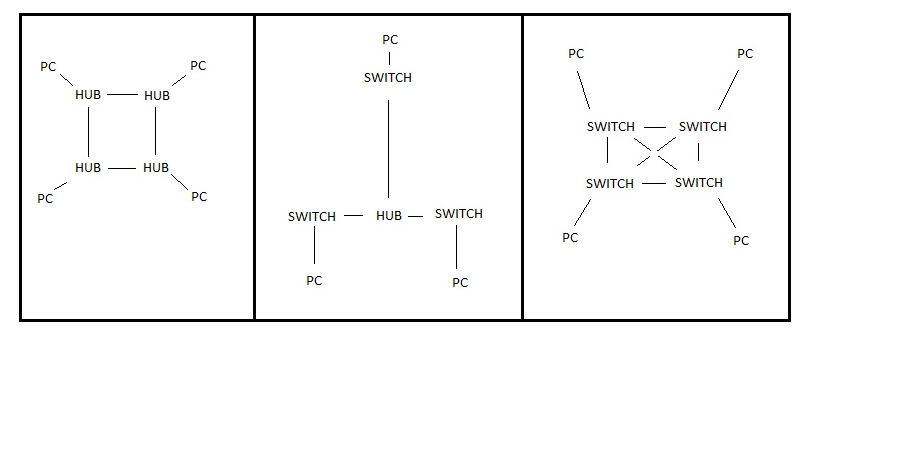
\includegraphics[scale=0.4]{images/listo.png}
    \caption{Imagen j}
    \label{fig:my_label}
\end{figure}

\section{Modelamiento (1) mediante software}
El primer modelo a representar utiliza los hardware de red correspondiente a HUBs y PCs como se muestra en la imagen k.
\begin{figure}
    \centering
    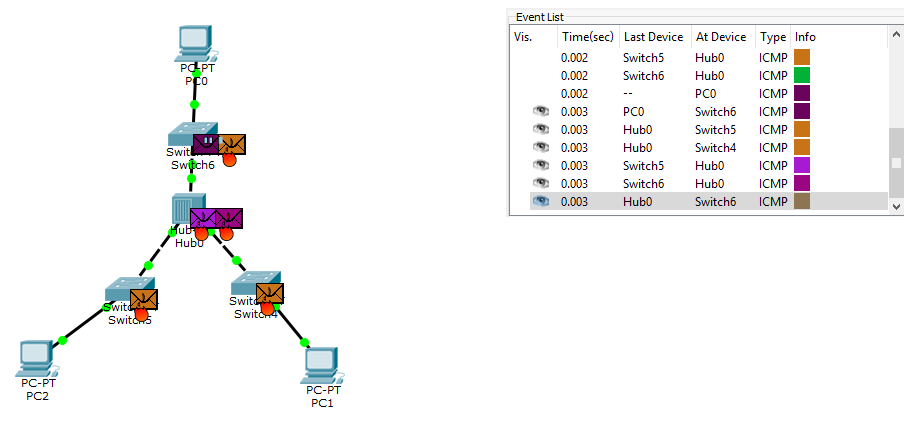
\includegraphics[scale=0.3]{images/ejemplo1.png}
    \caption{Imagen k}
    \label{fig:my_label}
\end{figure}
\\
\subsection{Observaciones}
El diseño mostrado en la figura k corresponde  a una topología estrella cuyo concentrador corresponde a un HUB el cual solo transmite información en un solo sentido (simplex).Como se logra apreciar los mensajes enviados entre los dispositivos colisionan debido a que no existe un orden temporal entre los participantes al momento de enviar los mensajes a la red provocando fallos en su recepción.
\\
\section{Modelamiento (2) mediante software}
El segundo modelo empleamos solo el uso de HUBs y PCs como se indica en la imagen L.
\\
\begin{figure}[h]
    \centering
    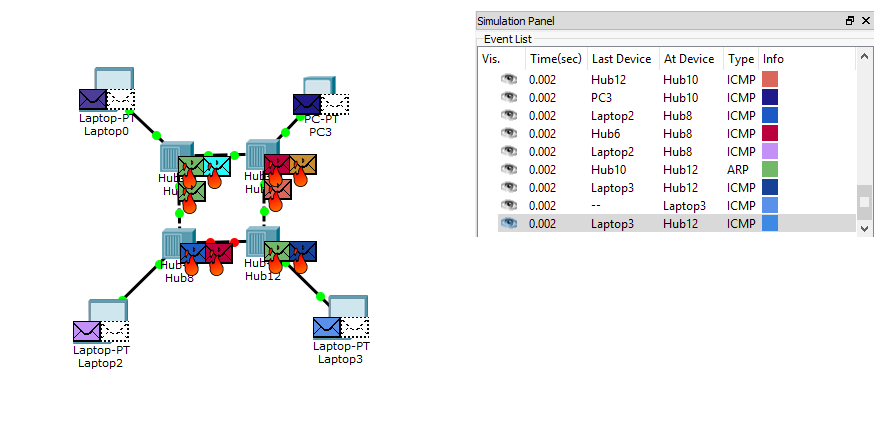
\includegraphics[scale=0.3]{images/EJEMPLO2 LIS.png}
    \caption{Imagen L}
    \label{fig:my_label}
\end{figure}
\subsection{Observaciones}
Esta conexión representa una topología de anillo, como se logra apreciar cada dispositivo envía paquete de datos unidireccionalmente, como se logra apreciar existe colisiones al momento de enviar mensajes entre todos los usuarios, para corregir estos problemas es necesario plantear un orden en los participantes de manera que los mensajes a emitir no colisiones al momento de llegar a destino.
\section{Modelamiento (3) mediante software}
Por ultimo, para este modelo solo hicimos  usos  de los dispositivos de red SWITCHs y PCs como se indica en la imagen Ñ.
\begin{figure}[h]
    \centering
    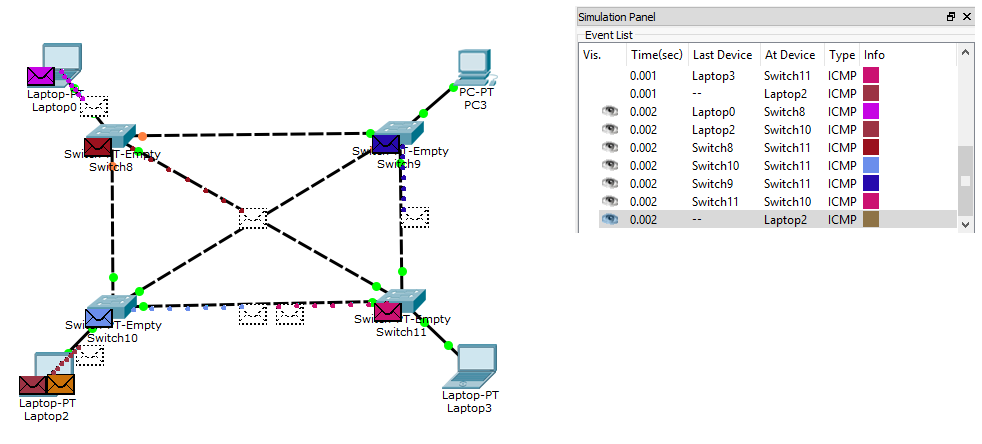
\includegraphics[scale=0.3]{images/EJEMPLO3 LIS.png}
    \caption{Imagen Ñ}
    \label{fig:my_label}
\end{figure}
\newpage
\subsection{Observaciones}
En este ultimo modelo se puede observar una topología del tipo malla, ya una vez realizado el montaje y emitir mensajes a todos los participantes presentes en la red se logra visualizar que no existen colisión en los paquetes de datos en la red, pero, si se logra ver que existen mensajes perdidos o que no llegan a su destino.
\\[0.4cm]
Cabe recordar que los switch trabajan a niveles de fullduplex por lo que el envió y recepción de mensajes puede ser posible entre los participantes, pero  presentar problemas cuando todos los participantes envían simultáneamente mensajes a todos los usuarios entre si ocasionando desfases en sus envíos y/o recepciones como también extravió de estos.
\newpage
\chapter{Actividad de investigación}
\section{Esquematización de  la sala de informática}
A continuación dispondré de un esquema a escala del levantamiento de red correspondiente a la sala de informática ubicada en el 5° piso de la escuela de ingeniería de la universidad Diego Portales (imagen a).
\\[0.2cm]
\begin{figure}[h]
    \centering
    \includegraphics[scale=0.5]{images/SalaInformatica.png}
    \caption{Imagen a}
    \label{fig:my_label}
\end{figure}
\\
El esquema planteado en la figura a, representa  la configuración reales que existe en la sala de informática, todos los computadores están conectados a una fuente de red que corresponde al dispositivo switch(imagen 1.1).
\begin{figure}
    \centering
    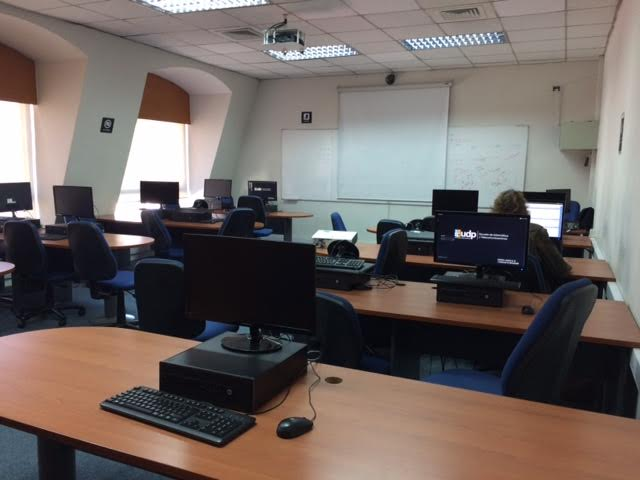
\includegraphics[scale=0.3]{images/apa.jpg}
    \caption{Imagen 1.1}
    \label{fig:my_label}
\end{figure}
\newpage
\section{Modelamiento de la sala de informática}
Presentación del modelo de la sala de informática mediante el uso del software packet tracer, imagen 1.
\begin{figure}[h]
    \centering
    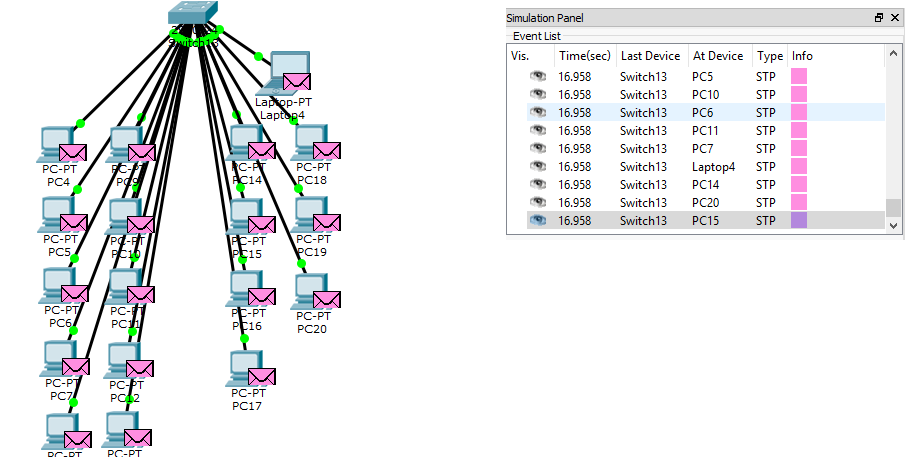
\includegraphics[scale=0.5]{images/inf111.png}
    \caption{Imagen 1}
    \label{fig:my_label}
\end{figure}
\\
Lo que se logra apreciar de la configuración modelada del laboratorio de informática es inicialmente que presenta una topología estrella que cuyo concentrador es un switch.
\\[0.2cm]
Ventajas: Solo se pueden conectar los dispositivos que se encuentren en la red, es decir, los dispositivos que  traten de unirse  a la red y  que además  presenten un IP distinto no podrán ni enviar ni recibir información en torno a esa red.
\\[0.2cm]
Desventajas:Si falla el switch cae toda la red.
\newpage
\section{Esquematización de la sala de telemática}
Ahora se presentara un esquema correspondiente a la sala de telemática ubicada en el 5° piso de la facultad de ingeniería(imagen 2)
\\[0.2cm]
\begin{figure}[h]
    \centering
    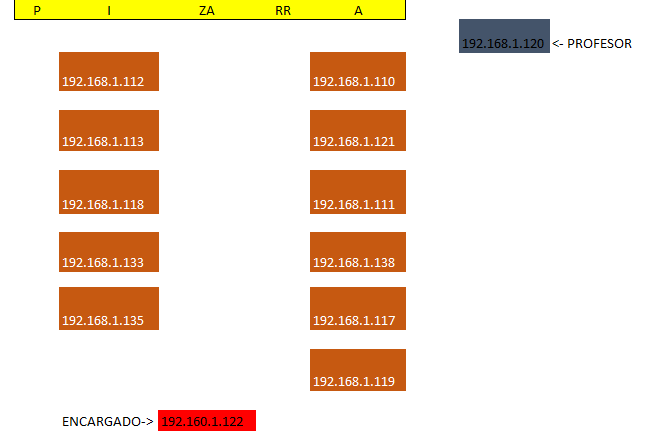
\includegraphics[scale=0.5]{images/telematica.png}
    \caption{Imagen 2}
    \label{fig:my_label}
\end{figure}
\\[0.2cm]
La representación del esquema representa el levantamiento real de la red de telemática como se muestra en la siguiente imagen (imagen 2.1).
\\[0.2cm]
\begin{figure}[h]
    \centering
    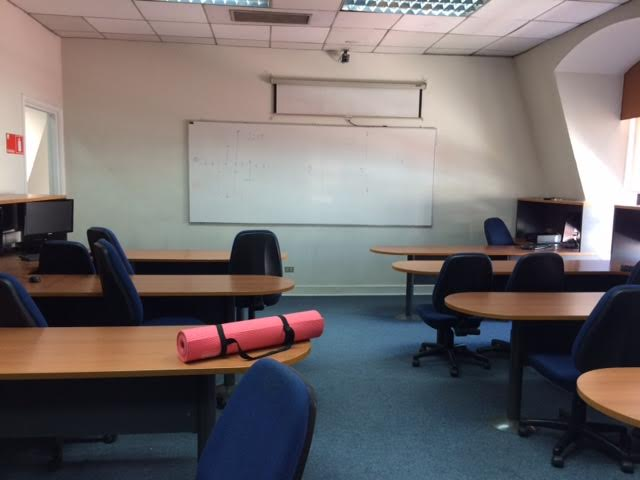
\includegraphics[scale=0.3]{images/unnamed.jpg}
    \caption{Imagen 2.1}
    \label{fig:my_label}
\end{figure}
\newpage
\section{Modelamiento de la sala de telemática}
Representación del modelo de la sala de telemática mediante el uso del software packet tracer,imagen w.
\\[0.2cm]
\begin{figure}[h]
    \centering
    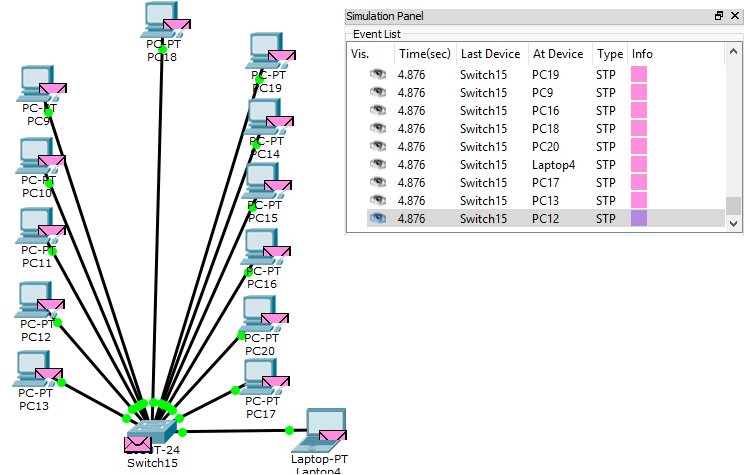
\includegraphics[scale=0.8]{images/telematica111.png}
    \caption{Imagen w}
    \label{fig:my_label}
\end{figure}
\\[0.4cm]
En cuanto al análisis de esta modelo, al igual que el modelo representado en la sala de informática,corresponde a una topología estrella cuyo concentrador corresponde a un switch.
\\[0.2cm]
En cuanto a rendimiento, al existir menor cantidad de dispositivos conectados puede haber un mejor rendimiento en el trafico de datos.
\newpage
\section{Esquema general de la red de ambas salas}
Una representación general del modelo de red uniendo ambas salas e indicando que las colisiones existentes son a nivel de broadcast,(imagen p).
\\[0.2cm]
\begin{figure}[h]
    \centering
    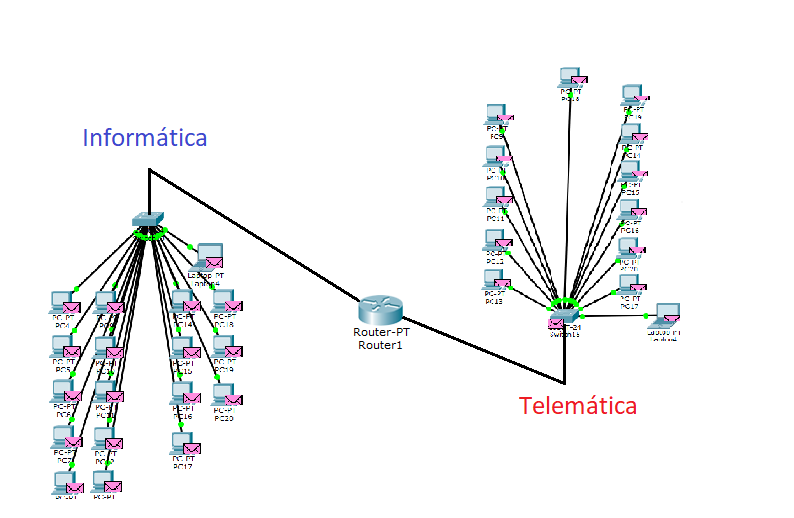
\includegraphics[scale=0.8]{images/general.png}
    \caption{Imagen p}
    \label{fig:my_label}
\end{figure}
\chapter{Cuestionario}
\begin{enumerate}
    \item ¿Cuáles son los diferentes equipos (con el nombre de los modelos) conectados en la red del laboratorio? 
    \item ¿Cuáles son las posibles ventajas y desventajas de las siguientes topologías? (Bus, estrella, malla, malla completa, anillo, árbol).
    \\ A continuación se detallara las ventajas y desventajas de las topologías de red:
    \\[0.1cm]
    a) Topología Bus:
    \begin{itemize}
        \item Ventaja: Una de las grandes ventajas de esta topología es principalmente su facilidad para instalarla y crecimiento, es la más económica con respecto a su implementación. 
        \item Desventaja: Su problema radica en que tiene longitudes de canal limitados, otro punto débil de esta red es que no es tolerante a fallas, es decir, un problema, por el más mínimo que sea en el canal, degrada toda la red, por ultimo y no menos importante es que este tipo de topología al agrandarla el desempeño disminuye.
    \end{itemize}
    b) Topología Estrella:
    \begin{itemize}
        \item Ventaja: Permite que los nodos se comuniquen entre si de manera conveniente, es mas tolerante con respecto a las fallas ya que si falla un computador esta sigue en funcionamiento, otro aspecto a considerar es que es mas organizada ya que esta centrada en el Switch o Hub.
        \item Desventaja: El numero de conexiones depende de la limitación del Switch o Hub, por otra parte, si falla el Switch la red entera falla  
    \end{itemize}
    c) Topología Malla:
    \begin{itemize}
        \item Ventaja: Es menos propenso a las interrupciones de comunicación, son confiables ya que si falla un nodo la red puede seguir en funcionamiento.
        \item Desventaja: El costo económico es el principal problema de este tipo de topología, debido a su alto uso de cables( en caso de usarlos), la disponibilidad del ancho de banda puede verse afectado por la cantidad de usuarios conectados a la red simultáneamente.
    \end{itemize}
    d) Topología Malla Completa:
    \begin{itemize}
        \item Ventaja: Es similar a las descripciones mencionadas en la topología malla solo que al estar completamente conectada se diferencia de la anterior en que esta no tiene interferencia de conexión, también, si falla un nodo en la red esta sigue funcionando ya que buscara otros caminos para hacer llegar el mensaje. 
        \item Desventaja: Al igual que en la topología malla su implementación es costosa en términos económicos.
    \end{itemize}
    e) Topología Anillo:
    \begin{itemize}
        \item Ventaja: Es simple con respecto a su arquitectura, es fácil de implementar. 
        \item Desventaja:Su longitud de canal es limitado en otras palabras se degrada si la red crece, tambien, esta topología es poco tolerante a fallas, si falla un nodo falla toda la red. 
    \end{itemize}
    \newpage
    f) Topología Arbol:
    \begin{itemize}
        \item Ventaja: Permite priorizar las comunicaciones de distintas computadoras, es como un conjunto de topologías estrella, esto implica que el numero de conexiones sea mas abundante. 
        \item Desventaja: Si la raíz principal de esta topología falla, se viene toda la red abajo. En relación a eso si falla un enlace un nodo hoja puede quedar aislado.
    \end{itemize}
    \item ¿Cuál es la diferencia entre dominio Broadcast y dominio de Colisión?
    \\El dominio de colisión se diferencia del dominio broadcast principalmente en las capas del modelo OSI en las cuales se mueves, es decir, el dominio de colisión trabaja en la capa 2 o superiores y el dominio broadcast o de difusión trabaja en la capa 3.
    \item¿En que facilitaría trabajar a nivel profesional con Packet Tracer? Argumente de manera completa.
    \\ Packet Tracer permite recrear un ambiente de red, es decir, es un simulador que permite detectar errores y corregir errores antes de una implementación, en este aspecto sería bastante útil ya que es de fundamental importancia modelar y asegurar que el trabajo realizado no presente fallas las cuales, en caso de no ser visible, seran muy difíciles de detectar para posteriormente corregir. 
    \\Otro aspecto importante es que este simulador, permite ver en detalle el desarrollo por capas del proceso de transmisión y recepción de un mensaje, esto es básicamente para comprobar que la red implementada funciona correctamente para los requerimientos dados.
    \item Dar un ejemplo de en el cual la topología lógica sea diferente a la topología física y argumentar el por qué es así.
    \\ Un caso en que la topología lógica y la física son diferentes es Ethernet, la cual tiene topología lógica Bus y topología física Estrella, esto se implemento para limitar sus interrupciones en la red. Otro ejemplo de topologías diferentes es Token Ring la cual tiene una topología lógica Anillo y Topología física Estrella, se atribuye al igual que lo anterior la limitación de interrupciones a la red ya que la topología estrella es mas tolerante a fallas, pero logicamente funciona distinto.

\end{enumerate}
\newpage
\chapter{Conclusión}
Luego de lo realizado en la experiencia practica del laboratorio correspondiente a la arquitectura de las redes, se obtuvo 
el aprendizaje necesario para corregir,detectar y realizar modelamientos de distintas topologías de red
mediante el uso del software packet tracer. Cabe destacar que una vez montado la estructura física se realizo distintos 
paquetes de datos entre los distintos usuarios de la red originada, dando inicio al envió y recepción de datos
que da origen a la topología lógica de la red. Mediante el modelamiento de distintas redes se adquirió el conocimiento 
necesario para diferenciar los distintos tipos de hardware existentes, su funcionamiento y como estos afectan el 
planteamiento de una red al momento de plantear la topología lógica, al igual que los dominios de broadcast y colisión que 
se puede generar al no crear una buena topología física con sus respectivos dispositivos.
\\[0.2cm]
Para el modelamiento de red correspondiente a la sala de informática y telemática, se realizo un estudio físico 
de la orientación de los computadores, la cantidad de estos mismos y sus respectivos IP asociados a cada uno de ellos.
También se logro identificar el tipo de topología predominante en cada una de las salas de laboratorio logrando 
identificar que el rendimiento de cada una de ellas solo se ve afectada por los tipos de switch a usar y la cantidad
de dispositivos con la que cada red cuenta.

En consecuencia ambas salas( telemática e informática) están conectadas a un router que no podemos identificar pero que 
si logramos evidenciar,logrando que cada sala presente sus propios dominios de colisión pero en una perspectiva mas amplia 
de la red logramos apreciar que ambas salas presentan un dominio de broadcast.
\\[0.2cm]
En consecuencia, la presente experiencia tiene como pilar principal la capacidad de crear un concepto claro de que las
topologías físicamente planteadas son a veces muy distintas a las topologías lógicas en cuanto al flujo de datos 
estemos hablando.

\begin{thebibliography}{0}
\bibitem{1}Dominio de colisión y broadcast. Recuperado de http://librosnetworking.blogspot.cl/2012/08/dominio-de-colision-dominio-de-broadcast.html
\bibitem{2}tipos de topologías. Recuperado de http://mariaangelicatorres.blogspot.cl/2013/04/tipos-de-topologias-ventajas-y.html
\end{thebibliography}
\listoffigures
\end{document}

